\documentclass[11pt,a4paper]{article}
\usepackage[utf8]{inputenc}
\usepackage[T1]{fontenc}

\usepackage[francais]{babel}
\usepackage[left=2cm,right=2cm,top=2cm,bottom=2cm]{geometry}
\usepackage{graphicx}
\usepackage{helvet}
\usepackage[hidelinks]{hyperref}
\usepackage{listings}
\usepackage{url}
\usepackage{xcolor}

\renewcommand{\familydefault}{\sfdefault}

\author{Dorian Burihabwa \and Aurelien Havet}
\title{Apply Java stack trace mining to a Stackoverflow dump to find most relevant questions against a stack trace index}
\date{02/12/2014}

\begin{document}
\maketitle
\tableofcontents
\section{Introduction}
Dans l'ingénierie logicielle, les bugs sont légions, et les rapports de crash sont des informations primordiales pour leurs réparations. Ils contiennent en particulier la pile d'appels de fonctions au moment du crash, dite stack trace, qui aide à la compréhension du contexte dans lequel a lieu l'erreur. Il est utile dans ce cas de pouvoir trouver une source d'information au sujet d'un crash ayant une stack trace similaire et proposant une solution pour éviter que le bug à l'origine de ce crash ne se repoduise.

StackOverflow\cite{SO} est un site dédié aux développeurs. Construit sous forme de blog, il permet à chacun de publier son problème afin que d'autres y répondent. S'il s'agit d'un bug logiciel, la stack trace correspondant à celui-ci peut avoir été publiée afin que d'autres développeurs puissent l'analyser et proposer une solution adéquate au problème. Post après post, ce site est devenu une vraie mine d'informations sur les erreurs logicielles rencontrées par la communauté informatique. Pouvoir trouver une question, et à postériori la solution associée, se rapprochant au maximum d'un problème rencontré par un développeur, est pour ce dernier un véritable gain de temps et de productivité.
\newline

Nous nous proposons ici de structurer et de stocker en base de données des stack traces extraites d'un dump des questions postées sur StackOverflow, afin de pouvoir en ressortir les candidates se rapprochant le plus d'une stack trace recherchée. L'idée est de pouvoir accéder de manière efficace et pertinente aux questions semblables au problème du développeur, et donc aux réponses proposées.

Ainsi, souhaitant établir les similarités entre différentes stack traces et donc mettre en exergue leurs points communs, nous avons modélisé celles-ci comme listes d'enchaînements de frames, une frame étant composée d'une méthode, un nom de fichier et d'un numéro de ligne, et correspond textuellement à une ligne de stack trace.

\section{Approche}

Le travail de départ consiste en l'extraction des données issues d'un dump de données de stackexchange librement accessible sur le site internet archive.org\cite{so-dump}.
Ces données représente l'ensembe des posts, tags et autre méta-données produites par l'ensemble des sites hébérgés par la plateforme StackExchange\cite{se}.
Parmi ces sites, StackOverflow présente l'ensemble de ses posts (questions et réponses) sous la forme d'un fichier XML d'une taille de 29 Go.
Son chargement complet en mémoire sur un poste de travail moyen est donc exclu.
Afin de rendre la recherhe dans le data set possible, le contenu du fichier \texttt{Posts.xml} sera traité sous forme de flux.
Dans un premier temps, nous nous intéressons uniquement à l'analyse des stack traces Java.
Son contenu sera alors filtré pour conserver les questions remplissant les critères suivants:
\newline

\begin{itemize}
	\item Avoir une réponse acceptée
	\item Porter le tag Java
	\item Contenir au moins une stack trace Java\newline
\end{itemize}

Les données filtrées seront directement injectées dans une base de données MySQL en prenant soin de minimiser la redondance en base de données.
\subsection{Parsing}

Notre étude se porte donc en premier lieu sur l'analyse des stack traces Java.
Ayant à notre disposition un parseur développé en Java adapté à cette recherche, notre choix sur la technologie à employer s'est naturellement orienté vers ce langage.
\newline

Le document original contenant les postes à traiter est une archive contenant un fichier XML.
Après décompression, ce fichier est d'une taille de 29 895 Mo.
Ce fichier est une suite de noeuds \texttt{<row>} (les posts) fils du noeud racine \texttt{<posts>}.
Sa taille se justifie par la présence de questions (bien ou mal formulées), de réponses (pertinentes ou non) mais surtout de méta-données, comme leur score, leur date de publication ou de dernière édition, ou encore l'identifiant de la réponse sélectionnée quand il y en a une.
\newline

Notre travail portant sur l'analyse de stack traces Java, un filtrage simple peut être mis en place pour réduire le fichier à une taille plus raisonable, et éviter ainsi le traitement inutile d'un grand nombre de posts.
À cette fin, nous avons développé un processeur de tag XML \texttt{XMLWriter}, procédant à la réécriture d'un fichier XML en filtrant les noeuds qui ne nous intéressent pas.
Ce travail de réduction produit un fichier XML d'une taille bien plus modeste : 128 Mo.
\newline

Arrivé à ce point, il est interressant de constater qu'un chargement complet en mémoire ne parait plus impossible.
Mais la taille désormais abordable du fichier en entrée est un resultat direct des conditions de filtrage que nous avons mises en place.
Travailler à extraire les données liées à un langage potentiellement plus populaire, ou l'ouverture à des posts autres que le questions, pourrait produire un fichier trop large pour envisager le chargement en RAM.
De plus, le traitement choisi pour ce projet porte principalement sur la transormation des données pour stockage dans une base de données SQL.
On peut donc profiter du processeur pour générer un fichier réduit comme base pour le travail de transformation, ou l'abandonner complètement afin traiter le fichier original et stocker directement nos données en base.

\subsection{Structuration des données}

Afin de répondre à notre besoin de persistence des stack traces analysées, nous optons pour une base de données MySQL.
Ce choix nous est apparu comme judicieux pour sa simplicité et la connaissance que nous avons de cette technologie.
\newline

Deux types de données nous intéressent : les questions et leurs stack traces.
Afin d'apporter une forme de normalisation, une restructuration s'impose.
Si les posts peuvent être conservés d'un seul tenant, les stack traces ne sont finalement qu'une suite de frames liées entre elles.
En particulier, l'idée de conserver les enchaînements de frames permet de détecter facilement les sous-suites communes entre différentes stack traces, telles des graphes ayant des chemins communs.
\newline

La figure \ref{fig:model} (page \pageref{fig:model}) illustre le modèle de données choisi pour le projet.
Une entité \texttt{Post} peut être liée à plusieurs entités \texttt{Stack} : cette relation est modélisée par une entité \texttt{PostStack} qui possède également comme attribut la position de l'entité \texttt{Stack} dans l'entité \texttt{Post}.
Une entité \texttt{Stack} quant à elle se compose d'entités \texttt{Link} qui représentent le passage d'une ligne de stack - fichier, fonction, ligne - à une autre.
Une telle transition pouvant potentiellement se retrouver dans différentes stack traces, nous avons modélisé le lien entre une entité \texttt{Stack} et une entité \texttt{Link} par une relation ManyToMany.
Enfin, une entité \texttt{Link} se compose donc de deux entités \texttt{Frame} : la parente et sa fille, la première représentant l'endroit d'où est appelée la seconde (i.e. à l'inverse de la lecture que nous faisons d'une stack trace : la fille précède la parente).
En tout bout de chaîne de ce diagramme, nous avons une entité \texttt{Frame} représentant simplement une ligne de stack trace : un nom de fichier, le nom de la méthode appelée, et le numéro de ligne d'appel de la méthode précédente.
Enfin l'entité \texttt{PostAnswer} permet de lier une question à ses réponses, dans l'idée d'une futur fonctionnalité de recherche des réponses associées à une stack trace, pour le développement de laquelle nous n'avons pas eu le temps nécessaire.
\newline

Comme pour le parser, un processeur a été développé pour traiter les tags XML reçus (voir la classe \texttt{SQLProcessor}).
Deux versions du processeur ont été créées.
Une première version se contentant d'insérer chaques frames et links sans se soucier de la duplication.
Une seconde version, beaucoup plus lente, vérifie la présence d'une frame avant de procéder à l'insertion, afin d'éviter la duplication des données identiques, et également de permettre une superposition de la représentation en mémoire des stack traces ayant des éléments communs.
\newline

\begin{figure}[h]
  \label{fig:model}
  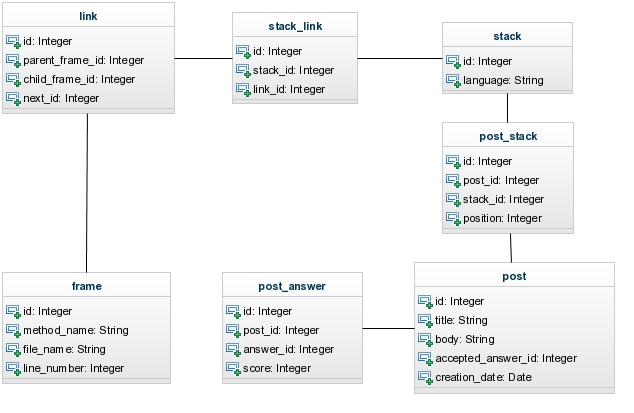
\includegraphics{stack_mining.jpeg}
  \caption{Modèle de données relationnel}
\end{figure}

\section{Résultats}

\begin{figure}[h]
\label{tbl:mysql}
\center
\begin{tabular} {|r|r|r|r|r|r|r|}
\hline
\textendash   & Posts & Stack traces & Frames & Links   & Taille (en Mo) & Dump (en Mo) \\
\hline
Non normalisé & 23090 & 29228        & 325329 & 296082  & 252 & 152\\
\hline
Normalisé     & 23090 & 29228        & 99841  & 296082  & 255 & 133\\
\hline
\end{tabular}
\caption{Stockage en base de données MySQL}
\end{figure}

Le tableau de la figure \ref{tbl:mysql} présente l'occupation en base des données analysées pour 2 versions du programme.
La première version est une version non normalisée listant le nombre de posts, de stack traces et de liens stockés en base de données.

Entre ces deux versions, on constate une nette diminution du nombre de frames enregistrées, de l'ordre de 70\%.
L'objectif étant de minimiser la redondance et faciliter la recherche en base de données sur base des index et de clés étrangères, cette évolution apparait comme un bénéfice.

Nous nous attendions également à apprécier une diminution du nombre de links, ce qui n'est pas le cas ici.
Cette anomalie nous a permis de déceler un bug de notre implémentation empêchant notre programme d'identifier les links déjà présents en base.
Nous avons donc écrit un test reproduisant ce bug, et fixé celui-ci, mais n'avons malheureusement pas eu le temps nécessaire à l'exécution d'une nouvelle analyse de notre tas de données.

Les deux dernières colonnes présentent respectivement l'occupation une fois chargé dans MySQL et la taille du fichier de dump SQL qui peut être généré à la fin du travail.

Ici encore, le résultat sur la taille de la base de données semble étrange, mais nous l'expliquons par l'ajout de contraintes d'intégrité entre nos tables avec l'utilisation de clés étrangères.
Celles-ci rajoute un coût non négligeable en terme de représentation en mémoire (par la création d'index entre les tables) et de performance en insertion (par la vérification des contraintes), mais promet de meilleures performances en sélection.
C'est d'ailleurs cette dernière que nous recherchons afin d'avoir un outil de recherche aussi efficace que possible.

Quant à la taille du dump, le gain sur celle-ci aurait sûrement été plus appréciable si il n'y avait pas eu de réplications des links.
\newline
 

\subsection{Exploitation des données}
Une fois les données importées en base de données, un certain nombre d'observations peuvent être faites.
Ces observations portent principalement sur les stack traces elles-mêmes.

On remarque que les stack traces enregistrées en base ont une longeur moyenne de 13,823 frames.
Cette longueur varie de 1 à 382 frames.

\subsection{Recherche de stack traces}
Un des objectifs potentiels de notre travail est la recherche de stack traces parmis celles accumulées par traitement du dump de Stackoverflow.

Au moment de l'écriture de ce rapport, il est possible de retrouver une stack trace entrée précédemment en la fournissant en entrée au programme.
Une amélioration intéressante serait l'extension à la recherche de sous-suites de frames similaires dans les stack traces.
À titre d'exemple, une recherche pour retrouver le premier post de la base de donnée est effectué en moins d'une demi-seconde (368 ms  en moyenne par recherche pour 100 recherches effectuées sur la même stack trace).

\begin{lstlisting}[caption=Sortie du programme de recherche dans les posts, breaklines=true,frame = single]
http://stackoverflow.com/questions/6816	Class file name must end with .class exception in Java Search
\end{lstlisting}

Fournir cette base de données comme système de recherche en y branchant un frontend plus agréable, par le web par exemple, offirait donc une alternative intéressante à la recherche purement textuelle disponible sur Stackoverflow, ou encore à l'utilisation des moteurs de recherches extérieurs comme Google.

\section{Améliorations possibles}

Trois axes d'amélioration sont envisageables afin d'obtenir des données plus fiables et plus rapidement :
\begin{enumerate}
\item La correction du parser
\item Le multi-threading de l'insertion en base de données
\item Optimisation de la base de donées\newline
\end{enumerate}

Une correction du parser permettrait d'obtenir de meilleur résultat lors de l'interprétation des frames.
En effet, les frames issues du dump proviennent d'entrée dans un champ de saisie libre, provoquant potentiellement la modification de la stack trace lors du formattage ou de l'édition du post.
Le premier changement qui pourrait être apporté serait une lecture plus efficace du numéro de ligne ou du nom du fichier lors de l'analyse de la frame.
Le parser utilisé pour ce projet introduisant parfois des caractères venus d'autres lignes dans ces réponses, réduisant à chaque fois un peu plus les possibilités de normalisation.
\newline

La seconde piste d'amélioration concerne le processus de transformation lui-même qui souffre actuellement de sa lenteur.
En effet, le travail de stockage des 23 000 stack traces représente une exécution de près de 12 heures sans normalisation.
La version normalisée double tout simplement le temps nécessaire en prenant un peu plus de 24 heures (89248884717900 ns) pour achever son éxecution - une différence de performance sur l'insertion vraisemblablement imputable à l'introduction des contraintes de clés étrangères, comme évoqué précédemment.

Séparer les responsabilité de parsing du document original et du stockage est une première étape.
Placer les résultats du parsing dans une file d'attente et laisser l'entité de stockage la vider régulièrement permettrait de libérer le document à parser.
Enfin, mulitplier le nombre d'entités en charge du stockage en fonction de la capacité de la machine hôte accélèrerait de manière significative le process.
Par soucis de simplicité et manque de temps, nous avons préféré ne pas déléguer l'insertion en base de données à plusieurs processus, évitant ainsi la complexification de l'implémentation.
Il est à noter qu'exécuter ce programme sur une machine dîte rapide - équipée d'un disque dur SSD et bien fournie en RAM - permettrait d'obtenir des résultats dans un temps plus raisonable.
\newline

Enfin, MySQL a été choisi comme premier choix pour sa facilité de maintenance.
Plus d'expertise dans l'optimisation du stockage et des requêtes sur ce SGBD aurait peut-être permis d'atteindre de meilleures performances.
Le choix d'un autre SGBD, ou d'une base de données NoSQL comme CouchDB\cite{sql-vs-nosql}, pourrait également permettre un gain de performances.

\section{Conclusion}
Nous avons ici réalisé l'analyse d'une quantité d'informations d'assez grande taille - près de 30 Go de données organisées en XML - et d'une certaine hétérogénéité - le corps de chaque post n'étant qu'une suite de caractères sans contrainte formelles - pour en tirer de l'information homogène - près de 30000 stack traces formalisées et persistées.

Ce tas de données organisées ouvre, au-delà des quelques statistiques présentées ici, des perspectives d'utilisation pour des recherches performantes de stack trace, ou de calcul de distance entre stack traces.

Notre implémentation\cite{sources} permet également d'envisager l'utilisation d'autres parsers, qui implémenteraient l'interface \texttt{StackTrackParserItf}, et qui seraient dédiés à la recherche de stack traces dans d'autres langages.

\bibliography{references}
\bibliographystyle{plain}
\end{document}
